% Auto-generated by experiments.analysis.generate_ci_plots --- do not edit.
\begin{figure}[H]
\centering
\adjustbox{max width=\textwidth}{%
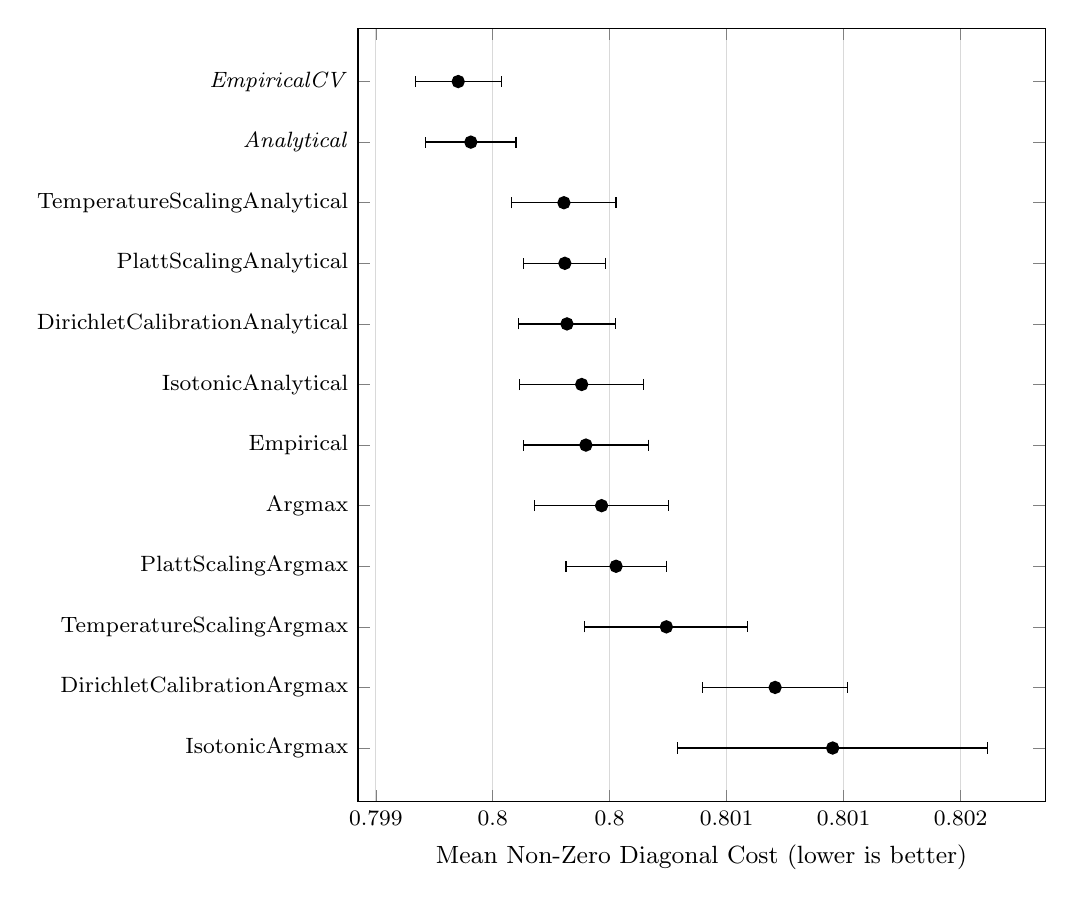
\begin{tikzpicture}
\begin{axis}[
    width=0.85\textwidth, height=11.40cm,
    xlabel={Mean Non-Zero Diagonal Cost (lower is better)},
    symbolic y coords={{EmpiricalCV},{Analytical},{TemperatureScalingAnalytical},{PlattScalingAnalytical},{DirichletCalibrationAnalytical},{IsotonicAnalytical},{Empirical},{Argmax},{PlattScalingArgmax},{TemperatureScalingArgmax},{DirichletCalibrationArgmax},{IsotonicArgmax}},
    ytick={{EmpiricalCV},{Analytical},{TemperatureScalingAnalytical},{PlattScalingAnalytical},{DirichletCalibrationAnalytical},{IsotonicAnalytical},{Empirical},{Argmax},{PlattScalingArgmax},{TemperatureScalingArgmax},{DirichletCalibrationArgmax},{IsotonicArgmax}},
    yticklabels={\textit{EmpiricalCV},\textit{Analytical},TemperatureScalingAnalytical,PlattScalingAnalytical,DirichletCalibrationAnalytical,IsotonicAnalytical,Empirical,Argmax,PlattScalingArgmax,TemperatureScalingArgmax,DirichletCalibrationArgmax,IsotonicArgmax},
    y dir=reverse,
    enlarge y limits=0.08,
    xmajorgrids=true,
    major grid style={draw=black!15, line width=0.3pt},
    scaled x ticks=false,
    xticklabel style={/pgf/number format/fixed, /pgf/number format/precision=3},
    tick label style={font=\footnotesize},
    label style={font=\small},
    every axis plot/.append style={thick},
]
\addplot[only marks, mark=*, mark size=2pt, color=black, error bars/x dir=both, error bars/x explicit, error bars/error bar style={color=black, line width=0.5pt}] coordinates { (0.799852,{EmpiricalCV}) +- (0.000183475,0) };
\addplot[only marks, mark=*, mark size=2pt, color=black, error bars/x dir=both, error bars/x explicit, error bars/error bar style={color=black, line width=0.5pt}] coordinates { (0.799906,{Analytical}) +- (0.00019296,0) };
\addplot[only marks, mark=*, mark size=2pt, color=black, error bars/x dir=both, error bars/x explicit, error bars/error bar style={color=black, line width=0.5pt}] coordinates { (0.800304,{TemperatureScalingAnalytical}) +- (0.000222498,0) };
\addplot[only marks, mark=*, mark size=2pt, color=black, error bars/x dir=both, error bars/x explicit, error bars/error bar style={color=black, line width=0.5pt}] coordinates { (0.800308,{PlattScalingAnalytical}) +- (0.00017561,0) };
\addplot[only marks, mark=*, mark size=2pt, color=black, error bars/x dir=both, error bars/x explicit, error bars/error bar style={color=black, line width=0.5pt}] coordinates { (0.800317,{DirichletCalibrationAnalytical}) +- (0.000207701,0) };
\addplot[only marks, mark=*, mark size=2pt, color=black, error bars/x dir=both, error bars/x explicit, error bars/error bar style={color=black, line width=0.5pt}] coordinates { (0.80038,{IsotonicAnalytical}) +- (0.000265909,0) };
\addplot[only marks, mark=*, mark size=2pt, color=black, error bars/x dir=both, error bars/x explicit, error bars/error bar style={color=black, line width=0.5pt}] coordinates { (0.800398,{Empirical}) +- (0.000266843,0) };
\addplot[only marks, mark=*, mark size=2pt, color=black, error bars/x dir=both, error bars/x explicit, error bars/error bar style={color=black, line width=0.5pt}] coordinates { (0.800465,{Argmax}) +- (0.00028664,0) };
\addplot[only marks, mark=*, mark size=2pt, color=black, error bars/x dir=both, error bars/x explicit, error bars/error bar style={color=black, line width=0.5pt}] coordinates { (0.800527,{PlattScalingArgmax}) +- (0.000214262,0) };
\addplot[only marks, mark=*, mark size=2pt, color=black, error bars/x dir=both, error bars/x explicit, error bars/error bar style={color=black, line width=0.5pt}] coordinates { (0.800742,{TemperatureScalingArgmax}) +- (0.000348452,0) };
\addplot[only marks, mark=*, mark size=2pt, color=black, error bars/x dir=both, error bars/x explicit, error bars/error bar style={color=black, line width=0.5pt}] coordinates { (0.801207,{DirichletCalibrationArgmax}) +- (0.000311069,0) };
\addplot[only marks, mark=*, mark size=2pt, color=black, error bars/x dir=both, error bars/x explicit, error bars/error bar style={color=black, line width=0.5pt}] coordinates { (0.801453,{IsotonicArgmax}) +- (0.000663325,0) };
\end{axis}
\end{tikzpicture}%
}
\caption{mammography: Non-Zero Diagonal Cost on TabICL (lower is better). Each dot is a strategy's mean over ten seeds with a $\pm 1$ SE horizontal bar; rows are sorted by mean, and the best strategy and any whose interval overlaps it are italicized.}%
\label{fig:ci-mammography-non-zero_diagonal_cost}
\end{figure}
